\documentclass[dvips, lscape]{foils}
%\documentclass[dvips, french]{slides}
\textwidth 18.5cm
\textheight 24.5cm 
\topmargin -1cm 
\oddsidemargin  -1cm 
\evensidemargin  -1cm

% Maths
\usepackage{amsfonts, amsmath, amssymb}

\newcommand{\coefbin}[2]{\left( 
    \begin{array}{c} #1 \\ #2 \end{array} 
  \right)}
\newcommand{\bbullet}{\bullet\bullet}
\newcommand{\bbbullet}{\bbullet\bullet}
\newcommand{\bbbbullet}{\bbbullet\bullet}
\newcommand{\Bcal}{\mathcal{B}}
\newcommand{\Ccal}{\mathcal{C}}
\newcommand{\Dcal}{\mathcal{D}}
\newcommand{\Ecal}{\mathcal{E}}
\newcommand{\Gcal}{\mathcal{G}}
\newcommand{\Mcal}{\mathcal{M}}
\newcommand{\Ncal}{\mathcal{N}}
\newcommand{\Pcal}{\mathcal{P}}
\newcommand{\Qcal}{\mathcal{Q}}
\newcommand{\Rcal}{\mathcal{R}}
\newcommand{\Hcal}{\mathcal{H}}
\newcommand{\Jcal}{\mathcal{J}}
\newcommand{\Lcal}{\mathcal{L}}
\newcommand{\Tcal}{\mathcal{T}}
\newcommand{\Ucal}{\mathcal{U}}
\newcommand{\Xcal}{\mathcal{X}}
\newcommand{\Zcal}{\mathcal{Z}}
\newcommand{\etabar}{\overline{\eta}}
\newcommand{\pibar}{\overline{\pi}}
\newcommand{\alphabf}{\mbox{\mathversion{bold}{$\alpha$}}}
\newcommand{\betabf}{\mbox{\mathversion{bold}{$\beta$}}}
\newcommand{\gammabf}{\mbox{\mathversion{bold}{$\gamma$}}}
\newcommand{\mubf}{\mbox{\mathversion{bold}{$\mu$}}}
\newcommand{\Pibf}{\mbox{\mathversion{bold}{$\Pi$}}}
\newcommand{\psibf}{\mbox{\mathversion{bold}{$\psi$}}}
\newcommand{\Sigmabf}{\mbox{\mathversion{bold}{$\Sigma$}}}
\newcommand{\taubf}{\mbox{\mathversion{bold}{$\tau$}}}
\newcommand{\thetabf}{\mbox{\mathversion{bold}{$\theta$}}}
\newcommand{\Abf}{{\bf A}}
\newcommand{\Ebf}{{\bf E}}
\newcommand{\Hbf}{{\bf H}}
\newcommand{\Ibf}{{\bf I}}
\newcommand{\Pbf}{{\bf P}}
\newcommand{\Sbf}{{\bf S}}
\newcommand{\mbf}{{\bf m}}
\newcommand{\ubf}{{\bf u}}
\newcommand{\vbf}{{\bf v}}
\newcommand{\wbf}{{\bf w}}
\newcommand{\nw}{n_{\wbf}}
\newcommand{\Nw}{N_{\wbf}}
\newcommand{\xbf}{{\bf x}}
\newcommand{\Xbf}{{\bf X}}
\newcommand{\Esp}{{\mathbb E}}
\newcommand{\Corr}{{\mathbb C}\mbox{orr}}
\newcommand{\Var}{{\mathbb V}}
\newcommand{\Ibb}{{\mathbb I}}
\newcommand{\Rbb}{\mathbb{R}}
\newcommand{\Vsf}{\mathsf{V}}
\newcommand{\Starsf}{\mathsf{*}}

% Couleur et graphiques
\usepackage{color}
\usepackage{graphics}
\usepackage{epsfig} 
\usepackage{pstcol}

% Texte
\usepackage{lscape}
\usepackage{../../../../Latex/fancyheadings, rotating, enumerate}
%\usepackage[french]{babel}
\usepackage[latin1]{inputenc}
%\definecolor{darkgreen}{cmyk}{0.5, 0, 0.5, 0.5}
%\definecolor{green}{cmyk}{0.5, 0, 0.5, 0.5}
\definecolor{orange}{cmyk}{0, 0.6, 0.8, 0}
\definecolor{jaune}{cmyk}{0, 0.5, 0.5, 0}
\newcommand{\textblue}[1]{\textcolor{blue}{#1}}
\newcommand{\textred}[1]{\textcolor{red}{#1}}
\newcommand{\textgreen}[1]{\textcolor{green}{ #1}}
\newcommand{\textlightgreen}[1]{\textcolor{green}{#1}}
%\newcommand{\textgreen}[1]{\textcolor{darkgreen}{#1}}
\newcommand{\textorange}[1]{\textcolor{orange}{#1}}
\newcommand{\textyellow}[1]{\textcolor{yellow}{#1}}
\newcommand{\refer}[2]{{\sl #1}}

% Sections
%\newcommand{\chapter}[1]{\centerline{\LARGE \textblue{#1}}}
% \newcommand{\section}[1]{\centerline{\Large \textblue{#1}}}
% \newcommand{\subsection}[1]{\noindent{\Large \textblue{#1}}}
% \newcommand{\subsubsection}[1]{\noindent{\large \textblue{#1}}}
% \newcommand{\paragraph}[1]{\noindent {\textblue{#1}}}
% Sectionsred
\newcommand{\chapter}[1]{
  \addtocounter{chapter}{1}
  \setcounter{section}{0}
  \setcounter{subsection}{0}
%  {\centerline{\LARGE \textblue{\arabic{chapter} - #1}}}
  {\centerline{\LARGE \textblue{#1}}}
  }
\newcommand{\section}[1]{
  \addtocounter{section}{1}
  \setcounter{subsection}{0}
%  {\centerline{\Large \textblue{\arabic{chapter}.\arabic{section} - #1}}}
  {\centerline{\Large \textblue{#1}}}
  }
\newcommand{\subsection}[1]{
  \addtocounter{subsection}{1}
%  {\noindent{\large \textblue{\arabic{chapter}.\arabic{section}.\arabic{subsection} - #1}}}
  {\noindent{\large \textblue{#1}}}
  }
\newcommand{\paragraph}[1]{\noindent{\textblue{#1}}}

%%%%%%%%%%%%%%%%%%%%%%%%%%%%%%%%%%%%%%%%%%%%%%%%%%%%%%%%%%%%%%%%%%%%%%
%%%%%%%%%%%%%%%%%%%%%%%%%%%%%%%%%%%%%%%%%%%%%%%%%%%%%%%%%%%%%%%%%%%%%%
%%%%%%%%%%%%%%%%%%%%%%%%%%%%%%%%%%%%%%%%%%%%%%%%%%%%%%%%%%%%%%%%%%%%%%
%%%%%%%%%%%%%%%%%%%%%%%%%%%%%%%%%%%%%%%%%%%%%%%%%%%%%%%%%%%%%%%%%%%%%%
\begin{document}
%%%%%%%%%%%%%%%%%%%%%%%%%%%%%%%%%%%%%%%%%%%%%%%%%%%%%%%%%%%%%%%%%%%%%%
%%%%%%%%%%%%%%%%%%%%%%%%%%%%%%%%%%%%%%%%%%%%%%%%%%%%%%%%%%%%%%%%%%%%%%
%%%%%%%%%%%%%%%%%%%%%%%%%%%%%%%%%%%%%%%%%%%%%%%%%%%%%%%%%%%%%%%%%%%%%%
%%%%%%%%%%%%%%%%%%%%%%%%%%%%%%%%%%%%%%%%%%%%%%%%%%%%%%%%%%%%%%%%%%%%%%
\landscape
\newcounter{chapter}
\newcounter{section}
\newcounter{subsection}
\setcounter{chapter}{0}
\headrulewidth 0pt 
\pagestyle{fancy} 
\cfoot{}
\rfoot{\begin{rotate}{90}{
      \hspace{1cm} \tiny S. Robin: Motif statistics
      }\end{rotate}}
\rhead{\begin{rotate}{90}{
      \hspace{-.5cm} \tiny \thepage
      }\end{rotate}}

%%%%%%%%%%%%%%%%%%%%%%%%%%%%%%%%%%%%%%%%%%%%%%%%%%%%%%%%%%%%%%%%%%%%%%
%%%%%%%%%%%%%%%%%%%%%%%%%%%%%%%%%%%%%%%%%%%%%%%%%%%%%%%%%%%%%%%%%%%%%%
\begin{center}
  \chapter{Motifs statistics }
  \vspace{0.5cm}
  \chapter{in biological sequences and networks}
  
  \vspace{1cm}
  {\large S. Robin} \\

   {UMR INA-PG / ENGREF / INRA, Paris} \\
   {Math�matique et Informatique Appliqu�es}
   
   {Statistics for Biological Sequences group}
   
\end{center}

\vspace{0.5cm}
\paragraph{Outline.} 
\begin{enumerate}
\item Some extensions and open questions for standard motifs
\item More complex motifs / Effective computations
\item Towards motifs in random graphs
\end{enumerate}

%%%%%%%%%%%%%%%%%%%%%%%%%%%%%%%%%%%%%%%%%%%%%%%%%%%%%%%%%%%%%%%%%%%%%%%%
%%%%%%%%%%%%%%%%%%%%%%%%%%%%%%%%%%%%%%%%%%%%%%%%%%%%%%%%%%%%%%%%%%%%%%%%
\newpage
\section{(Brief) motivation}
%%%%%%%%%%%%%%%%%%%%%%%%%%%%%%%%%%%%%%%%%%%%%%%%%%%%%%%%%%%%%%%%%%%%%%%%
%%%%%%%%%%%%%%%%%%%%%%%%%%%%%%%%%%%%%%%%%%%%%%%%%%%%%%%%%%%%%%%%%%%%%%%%

Motif statistics are part of the standard tools of genomic sequences
analysis. \\
The search for motifs (short sequences of nucleotides {\tt a}, {\tt
  c}, {\tt g}, {\tt t}) having specific functions or unexpected
behavior is a way to understand the genetic information.

\paragraph{Some typical questions:} (cf. Book)
\begin{description}
\vspace{-0.5cm}
\item[Blind search:] In a new genome $\Sbf$, consider all the words of
  length $k$ ($4^k$ possible words) and detect the unexpectedly
  frequent (or rare) ones. \\
  Ex: palindromes of length 6 or 8 are avoided in {\sl E. coli}'s
  genome.
%\vspace{-0.5cm}
\item[Distribution along the genome:] Given a motif with known
  function, detect the region of the genome where its occurrences are
  'too' abundant (or rare). \\
  Ex: Distribution of the CHI sites in bacterial genomes.
%\vspace{-0.5cm}
\item[Structured motif:] Given a general specified structure and some
  regions where the motif is expected to occur, detect the motif that
  actually fulfils the biological function. \\
  Ex: Detection of promoter motifs.
\end{description}

%%%%%%%%%%%%%%%%%%%%%%%%%%%%%%%%%%%%%%%%%%%%%%%%%%%%%%%%%%%%%%%%%%%%%%%%
\newpage
\section{Need for a model}
%%%%%%%%%%%%%%%%%%%%%%%%%%%%%%%%%%%%%%%%%%%%%%%%%%%%%%%%%%%%%%%%%%%%%%%%
These questions can only be answered if we know what to expect. The
role of the statistical model is to describe the expected behaviour.

\paragraph{Most popular models.}
\vspace{-0.5cm}
\begin{description}
\item[Markov chain (MC):] The observed sequence $\Sbf = (X_1, X_1, ...
  X_n)$ is supposed to be generated by a stationary MC of order $m$
  (MC$m$) with transition $\Pibf$ and stationary distribution
  $\mubf$. \\
  Exact results about the occurrence probability, the distribution of
  the number of occurrences (count $\Nw$), the distance between
  occurrences are available. \\
  Many approximations of the distribution of the counts
  (Gaussian, compound Poisson, binomial, ...) are used in practice.
\item[Compound Poisson process:] The sequence is seen as a continuous
  line. The motif occurs in clumps. The clumps occur according to a
  Poisson process with intensity $\lambda$. The clump sizes are iid
  with geometric distribution $\Gcal(1-a)$, where $a$ is the
  {\em overlapping probability} of the motifs.
\end{description}


%%%%%%%%%%%%%%%%%%%%%%%%%%%%%%%%%%%%%%%%%%%%%%%%%%%%%%%%%%%%%%%%%%%%%%%%
%%%%%%%%%%%%%%%%%%%%%%%%%%%%%%%%%%%%%%%%%%%%%%%%%%%%%%%%%%%%%%%%%%%%%%%%
\newpage
\chapter{Extensions and open questions for standard motifs}
%%%%%%%%%%%%%%%%%%%%%%%%%%%%%%%%%%%%%%%%%%%%%%%%%%%%%%%%%%%%%%%%%%%%%%%%
%%%%%%%%%%%%%%%%%%%%%%%%%%%%%%%%%%%%%%%%%%%%%%%%%%%%%%%%%%%%%%%%%%%%%%%%

%%%%%%%%%%%%%%%%%%%%%%%%%%%%%%%%%%%%%%%%%%%%%%%%%%%%%%%%%%%%%%%%%%%%%%%%
\bigskip
\section{Large deviation for the count}
%%%%%%%%%%%%%%%%%%%%%%%%%%%%%%%%%%%%%%%%%%%%%%%%%%%%%%%%%%%%%%%%%%%%%%%%

In a sequence $\Sbf$ of length $\ell$, the word $\wbf$ occurs
$\nw$ times. We want to evaluate 
$$
\Pr\{\Nw \geq \nw\}
$$
especially in the case where the observed count is much larger than expected:
$$
\nw \gg \Esp \Nw.
$$
The large deviation approach is quite natural.

The PhD of G. Nuel (Evry, 2001) and P. Pudlo (Lyon, 2004) both propose
approximations for $\Pr\{\Nw \geq \nw \}$ and the joint probability $\Pr
\{ (N_{\wbf_i} \geq n_{\wbf_i})_{i=1, 2, ...})\}$ in the homogenous
MC$m$ framework. 

The practical implementation requires the calculation of the largest
eigenvalue of a matrix of size $m^k$.

% %%%%%%%%%%%%%%%%%%%%%%%%%%%%%%%%%%%%%%%%%%%%%%%%%%%%%%%%%%%%%%%%%%%%%%%%
% \newpage
% \section{Heterogenous Markov models}
% %%%%%%%%%%%%%%%%%%%%%%%%%%%%%%%%%%%%%%%%%%%%%%%%%%%%%%%%%%%%%%%%%%%%%%%%

%%%%%%%%%%%%%%%%%%%%%%%%%%%%%%%%%%%%%%%%%%%%%%%%%%%%%%%%%%%%%%%%%%%%%%%%
\newpage
\section{Comparing genomes}
%%%%%%%%%%%%%%%%%%%%%%%%%%%%%%%%%%%%%%%%%%%%%%%%%%%%%%%%%%%%%%%%%%%%%%%%

\paragraph{Comparative genomics.}
The number of occurrences of the word $\wbf$ is $N_1$ in sequence
$\Sbf_1$ (length $\ell_1$) and $N_2$ in sequence $\Sbf_2$ (length
$\ell_2$).  Is $\wbf$ 'more exceptional' in $\Sbf_1$ than in $\Sbf_2$?

\paragraph{Example.} If $N_1 \sim \Pcal(\lambda_1)$ and $N_2 \sim
\Pcal(\lambda_2)$ then, denoting $N_+ = N_1+N_2$,
$$
N_1 \;|\; N_+ \sim \Bcal\left(N_+,
  \frac{\lambda_1}{\lambda_1+\lambda_2} \right).
$$
The parameter $\lambda_i$ accounts for the length $\ell_i$ and the
composition of $\Sbf_i$.

\paragraph{Exercise.} Same problem with compound Poisson distribution
(for overlapping words):
\begin{enumerate}
\vspace{-0.5cm}
\item Compare the number of clumps.
\vspace{-0.5cm}
\item Compare the clumps sizes.
\end{enumerate}

%%%%%%%%%%%%%%%%%%%%%%%%%%%%%%%%%%%%%%%%%%%%%%%%%%%%%%%%%%%%%%%%%%%%%%%%
\newpage
\paragraph{Mosaic project.} Comparison of bacterial genome based on
multiple genome alignment ({\sl Chiapello \ al., 05}). \\
Example: The comparison of 3 strains of {\sl E. coli} (\textblue{CFT},
\textred{Sakai} and \textgreen{K12})

\hspace{-1.6cm}
\begin{tabular}{ll}
  \paragraph{Backbone and loops.}
  &
  \paragraph{Motifs statistics.} 
  \\
  \\
  Backbone = common parts & Comparison backbone / loops \\
  Loops = specific parts & for a specific strain (K12). \\
  \begin{tabular}{p{10cm}}
    \\
    \epsfig{file = ../Figures/Backbone-Loops.ps, clip=, bbllx=190,
      bblly=120, bburx=400, bbury=340} \\
    %\\
    (Source: EL Karoui, 06)
  \end{tabular}
  &
  \begin{tabular}{p{12cm}}
    \begin{enumerate}
    \item CHI sites are much more frequent in the backbone than in the
      loops;
    \item Palindromes are more frequent in the loops than in the
      backbone;
    \item Palindromes are yet avoided in the older loops.
    \end{enumerate}
  \end{tabular}
\end{tabular}

%%%%%%%%%%%%%%%%%%%%%%%%%%%%%%%%%%%%%%%%%%%%%%%%%%%%%%%%%%%%%%%%%%%%%%%%
\newpage
\section{What about statistics?}
%%%%%%%%%%%%%%%%%%%%%%%%%%%%%%%%%%%%%%%%%%%%%%%%%%%%%%%%%%%%%%%%%%%%%%%%

\paragraph{Approximation  + Estimation.}
Most distributions used in practice ($\Ncal$, $\Pcal$, $\Ccal\Pcal$)
only approximate the exact distribution under an MC$m$ model.  

The parameter $\theta$ of the approximated distribution depends on the
true transition matrix $\Pibf$.

$\Pibf$ is actually estimated by $\widehat{\Pibf}$ and a plug-in
version $\widehat{\theta}$ of $\theta$ is used for calculation.

Denoting $\Qcal$ the true distribution and $\Pcal(\theta)$ the
approximation, we have
$$
d(\Qcal, \Pcal(\widehat{\theta})) \leq 
\underset{\mbox{Approximation}}{\underbrace{d(\Qcal, \Pcal(\theta))}} 
+ 
\underset{\mbox{Estimation}}{\underbrace{d(\Pcal(\theta),
    \Pcal(\widehat{\theta}))}}. 
$$

Only {\sl Prum \& al. and Schbath (95)} take into account the fact
that $\widehat{\Pibf}$ and $\nw$ are observed on the same sequence.

%%%%%%%%%%%%%%%%%%%%%%%%%%%%%%%%%%%%%%%%%%%%%%%%%%%%%%%%%%%%%%%%%%%%%%%%
\newpage
\subsection{What can we do?}

\bigskip
\paragraph{Pangloss:} The genome of {\sl B. subtilis} is the one we
observe. There is no theoretical $\Pibf$, only $\widehat{\Pibf}$ makes
sense.

\bigskip
\paragraph{Panic:} Simulations in the MC$m$ framework show that the
estimation error may be much larger than the approximation error,
especially for large $m$. \\
$\Longrightarrow$ never consider MC$m$ with $m$ larger than 3 or 4.

\bigskip
\paragraph{But.} Biological sequences are not Markov chains. The
variability between different copies of the genome of a same species
has nothing to do with the variability between different paths of a
Markov chain.

\bigskip
Some bacterial genomes {\sl E. coli} (?) have been sequenced several
times: this variability can be studied now.

%%%%%%%%%%%%%%%%%%%%%%%%%%%%%%%%%%%%%%%%%%%%%%%%%%%%%%%%%%%%%%%%%%%%%%%%
%%%%%%%%%%%%%%%%%%%%%%%%%%%%%%%%%%%%%%%%%%%%%%%%%%%%%%%%%%%%%%%%%%%%%%%%
\newpage
\chapter{More complex motifs}
%%%%%%%%%%%%%%%%%%%%%%%%%%%%%%%%%%%%%%%%%%%%%%%%%%%%%%%%%%%%%%%%%%%%%%%%
%%%%%%%%%%%%%%%%%%%%%%%%%%%%%%%%%%%%%%%%%%%%%%%%%%%%%%%%%%%%%%%%%%%%%%%%

%%%%%%%%%%%%%%%%%%%%%%%%%%%%%%%%%%%%%%%%%%%%%%%%%%%%%%%%%%%%%%%%%%%%%%%%
\bigskip
\section{Structured motifs}
%%%%%%%%%%%%%%%%%%%%%%%%%%%%%%%%%%%%%%%%%%%%%%%%%%%%%%%%%%%%%%%%%%%%%%%%

%%%%%%%%%%%%%%%%%%%%%%%%%%%%%%%%%%%%%%%%%%%%%%%%%%%%%%%%%%%%%%%%%%%%%%
\subsection{Promoter motifs} 

Structured motifs where the polymerase binds to DNA
$$
\begin{pspicture}(20, 2.5)(0, -2.5)
  \psline[linewidth=0.05, linestyle=dashed, linecolor=black]{<-|}(0,
  1.2)(14.2, 1.2) 
  \rput[B]{0}(6.85, 1.4){$\simeq$ 100 bps}

  \psline[linewidth=0.1, linecolor=black](0, 0)(3.3, 0)
  \rput[B]{0}(4, -0.1){\fbox{\rule[-0.2cm]{0cm}{0.8cm}$\;\wbf_1\;$}}
  \psline[linewidth=0.1, linecolor=black](4.7, 0)(7.3, 0)
  \rput[B]{0}(8, -0.1){\fbox{\rule[-0.2cm]{0cm}{0.8cm}$\;\wbf_2\;$}}
  \psline[linewidth=0.1, linecolor=black](8.7, 0)(14.2, 0)
  \rput[B]{0}(17, -0.1){\fbox{\rule[-0.2cm]{0cm}{0.8cm}\qquad gene\qquad}}
  
  \psline[linewidth=0.05, linestyle=dashed, linecolor=black]{<->}(4.7,
  -1)(7.2, -1) 
  \rput[B]{0}(5.95, -2){16 bps $\leq d \leq$ 18 bps}
\end{pspicture}
$$
Which structured motifs occur almost ({\sl too} ?) systematically
in upstream regions of the genes of a given species?

%%%%%%%%%%%%%%%%%%%%%%%%%%%%%%%%%%%%%%%%%%%%%%%%%%%%%%%%%%%%%%%%%%%%%%%%
\newpage
\section{A first approximation}
%%%%%%%%%%%%%%%%%%%%%%%%%%%%%%%%%%%%%%%%%%%%%%%%%%%%%%%%%%%%%%%%%%%%%%%%
\paragraph{Difficulty:} Complexity of the overlapping structure of structured
motif 
$$
\begin{pspicture}(11, 1.75)(0, 0.75)
  \rput[B]{0}(1, 1){$\mbf = \framebox{\quad$\wbf_1$\quad}$}
  \psline[linewidth=0.1, linecolor=black]{<->}(3.2, 1.1)(8.7, 1.1)
  \rput[B]{0}(10, 1){\framebox{\quad$\wbf_2$\quad}}
  \rput[B](6, 1.3){$d$}
\end{pspicture}
$$
impossible to calculate the exact distribution of the waiting time
with the classical method (generating function).

\paragraph{Approximation} ({\em R. \& al, 02})
\vspace{-0.5cm}
\begin{enumerate}
\item Probability for $\mbf$ to occur at a given position (using the
  distribution of the distances): $ \mu(\mbf)$ 
\item Approximation of order 0 (geometric) does not work (simulations) :
  $$
  \gamma(\mbf) = \Pr \left\{ N(\wbf) \geq 1 \right\}
  \approx
  1 - [1 - \mu(\mbf)]^{\ell - |\mbf| + 1}.
  $$
\item Approximation of order 1 $\left(\mu_1(\mbf) = \Pr\{\mbf \mbox{
      at }x | \mbf \mbox{ not at } x-1\}\right)$:
  $$
  \gamma(\mbf) \approx 1 - [1 - \mu(\mbf)] [1 -
  \mu_1(\mbf)]^{\ell-|\mbf|}
  $$
\end{enumerate}


%%%%%%%%%%%%%%%%%%%%%%%%%%%%%%%%%%%%%%%%%%%%%%%%%%%%%%%%%%%%%%%%%%%%%%%%
\newpage
\section{Exact distribution of the waiting time}
%%%%%%%%%%%%%%%%%%%%%%%%%%%%%%%%%%%%%%%%%%%%%%%%%%%%%%%%%%%%%%%%%%%%%%%%

\paragraph{Decomposition of the waiting time.} $\wbf_2 =
\square, \wbf_2 = \bigcirc$:

$$
\epsfig{file=../Figures/WaitingStructuredMotif.ps, clip=, bbllx=112,
  bblly=610, bburx=470, bbury=700, width=18cm}
$$
\vspace{-0.5cm}
To get an occurrence of $\mbf$ we have to
\begin{itemize}
\vspace{-0.5cm}
\item wait for an occurrence of $\wbf_1$,
\vspace{-0.5cm}
\item followed by an occurrence of $\wbf_2$
\vspace{-0.5cm}
\item and check if $\wbf_2$ occurs at an admissible distance of
  $\wbf_1$.
\end{itemize}
The number of failure before success has a geometric distribution. \\
({\sl Stefanov, Schbath, R., 05})

%%%%%%%%%%%%%%%%%%%%%%%%%%%%%%%%%%%%%%%%%%%%%%%%%%%%%%%%%%%%%%%%%%%%%%%%
\newpage
Denote
\begin{description}
\vspace{-0.5cm}
\item[$T_{ij}$, $i,j\in\{1,2\}$:] the waiting time to reach pattern
  $\wbf_j$ from pattern $\wbf_i$;
\vspace{-0.5cm}
\item[$T_j^{(s)}$:] the waiting time to reach pattern $\wbf_j$ from
  state $s$;
\vspace{-0.5cm}
\item[$r_{ij}$, $i,j\in\{1,2\}$:] the probability that the first
  pattern from the family $\mathcal{W}$ to be reached is $w_j$, given
  we start from pattern $\wbf_i$;
\vspace{-0.5cm}
\item[$S_{12}$] (resp. $F_{12}$) = $X_{12}$ conditional to a success
  (resp. failure).
\end{description}
The generating functions of the waiting time until $\mbf$ starting from
letter $s$ and from word $\wbf_2$ are
\begin{eqnarray*}
G_{\mbf}^{(s)}(t)
&=& \frac{  r_{12} \, q_S \, G_{T_{1}^{(s)}}(t) \,G_{S_{12}}(t)}
        {\left[1- (1-r_{12}) G_{X_{11}}(t) \right]
         \left[1-(1-q_S) \frac{r_{12} \, G_{T_{21}}(t) \, G_{F_{12}}(t)}
                                     {1- (1-r_{12}) G_{X_{11}}(t)}                      
         \right]},
 \\
G_{\mbf}^{(\wbf_2)}(t)
&=& \frac{  r_{12} \, q_S \, G_{T_{21}}(t) \, G_{S_{12}}(t)}
        {\left[1- (1-r_{12}) G_{X_{11}}(t) \right] \left[1-(1-q_S)
            \frac{r_{12}\, G_{T_{21}}(t) \, G_{F_{12}}(t)} 
            {1- (1-r_{12}) G_{X_{11}}(t)} \right]}.
\end{eqnarray*}
$G_{\mbf}$ gives the probability $\gamma_{\ell}(\mbf)$ that
a sequence with length $\ell$. \\

%%%%%%%%%%%%%%%%%%%%%%%%%%%%%%%%%%%%%%%%%%%%%%%%%%%%%%%%%%%%%%%%%%%%%%%%
\newpage 
\paragraph{Motif detection.} Among $n$ sequences with same length, the number $N$ of sequences
containing $\mbf$ has a binomial distribution: $N \sim \Bcal(n,
\gamma_{\ell}(\mbf))$.

\hspace{-2cm}
\begin{tabular}{ll}
  \begin{tabular}{p{4cm}}
    \paragraph{Promoters in {\sl B. subtilis}:} \\
    \\
    regions of 100 bps \\
    upstream of $n=131$ genes (biologically
    validated) \\
    \\
    $p$-value $< 10^{-16}$ \\
    \\
    (putative alignment) \\
  \end{tabular}
  &
  \begin{tabular}{l}
    {\small
      \begin{tabular}{lclccc}
        \multicolumn{1}{c}{$\wbf_1$} & $(d_1:d_2)$ & \multicolumn{1}{c}{$\wbf_2$} & $N$ &
        $\gamma_{\ell}(\mbf)$ & $p$-value \\ 
        \hline 
        {\tt \ ttgactt}    & (16:18) & {\tt \ \ ataataa}  & 3 & 1.16\,$10^{-5}$ & 5.77\,$10^{-10}$\\
        {\tt \ \ tgactt}   & (16:18) & {\tt \ \ ataataa}  & 3 & 3.02\,$10^{-5}$ & 1.00\,$10^{-8}$\\
        {\tt \ ttgactt}    & (16:18) & {\tt \ \ atactaa}  & 2 & 4.01\,$10^{-6}$ & 1.37\,$10^{-7}$\\
        {\tt \ \ tgactt}   & (16:18) & {\tt \ \ atactaa}  & 2 & 1.04\,$10^{-5}$ & 9.18\,$10^{-7}$\\
        {\tt \ ttgaca}     & (16:18) & {\tt \ tataatg}    & 2 & 1.60\,$10^{-5}$ & 2.18\,$10^{-6}$\\
        {\tt \ ttgaca}     & (16:18) & {\tt \ tatatta}    & 2 & 2.36\,$10^{-5}$ & 4.75\,$10^{-6}$\\
        {\tt \ ttgact}     & (16:18) & {\tt \ tatact}     & 2 & 2.38\,$10^{-5}$ & 4.81\,$10^{-6}$\\
        {\tt \ ttgaca}     & (16:18) & {\tt \ tataata}    & 2 & 2.48\,$10^{-5}$ & 5.23\,$10^{-6}$\\
        {\tt \ ttgaca}     & (16:18) & {\tt atataat}      & 2 & 2.74\,$10^{-5}$ & 6.39\,$10^{-6}$\\
        {\tt \ \ tgacttt}  & (16:18) & {\tt \ \ \ taataa} & 2 & 3.63\,$10^{-5}$ & 1.12\,$10^{-5}$\\
        {\tt \ \ \ gacttt} & (16:18) & {\tt \ \ \ taataa} & 2 & 1.06\,$10^{-4}$ & 9.52\,$10^{-5}$\\
        {\tt gttgaca}      & (16:18) & {\tt \ tataata}    & 1 & 3.89\,$10^{-6}$ & 5.09\,$10^{-4}$\\
        {\tt gttgaca}      & (16:18) & {\tt atataat}      & 1 & 4.30\,$10^{-6}$ & 5.63\,$10^{-4}$\\
        {\tt \ ttgacac}    & (16:18) & {\tt \ \ ataataa}  & 1 & 4.88\,$10^{-6}$ & 6.39\,$10^{-4}$\\
        {\tt gttgac}       & (16:18) & {\tt ctataat}      & 1 & 4.88\,$10^{-6}$ & 6.39\,$10^{-4}$\\
      \end{tabular}
      }
  \end{tabular}
\end{tabular}

%%%%%%%%%%%%%%%%%%%%%%%%%%%%%%%%%%%%%%%%%%%%%%%%%%%%%%%%%%%%%%%%%%%%%%%%
%%%%%%%%%%%%%%%%%%%%%%%%%%%%%%%%%%%%%%%%%%%%%%%%%%%%%%%%%%%%%%%%%%%%%%%%
\newpage
\section{Effective computation of the distributions}
%%%%%%%%%%%%%%%%%%%%%%%%%%%%%%%%%%%%%%%%%%%%%%%%%%%%%%%%%%%%%%%%%%%%%%%%
%%%%%%%%%%%%%%%%%%%%%%%%%%%%%%%%%%%%%%%%%%%%%%%%%%%%%%%%%%%%%%%%%%%%%%%%

%%%%%%%%%%%%%%%%%%%%%%%%%%%%%%%%%%%%%%%%%%%%%%%%%%%%%%%%%%%%%%%%%%%%%%%%
\bigskip
\subsection{Automata}
%%%%%%%%%%%%%%%%%%%%%%%%%%%%%%%%%%%%%%%%%%%%%%%%%%%%%%%%%%%%%%%%%%%%%%%%

\paragraph{Example.} Automat counting the overlapping occurrences of
$\wbf = {\tt aba}$:

$$
% \epsfig{file = ../Figures/Automat-abab.ps, clip=, bbllx=45,
%   bblly=152, bburx=535, bbury=344}
\epsfig{file = ../Figures/Automat-aba.ps, clip=, bbllx=80,
  bblly=435, bburx=540, bbury=650}
\vspace{-1.5cm} $$
(Source: Nicod�me, 02)

%%%%%%%%%%%%%%%%%%%%%%%%%%%%%%%%%%%%%%%%%%%%%%%%%%%%%%%%%%%%%%%%%%%%%%%%
\newpage
\subsection{Combinatorial tools}

Such automaton can be build automatically for (even complex) regular
motifs. 

\paragraph{Exact distribution.}
The associated generating function is derived at the same time
(cf. RegExpCount package, Nicod�me, 01).

%%%%%%%%%%%%%%%%%%%%%%%%%%%%%%%%%%%%%%%%%%%%%%%%%%%%%%%%%%%%%%%%%%%%%%%%
\vspace{1cm}
\subsection{Finite Markov chains imbedding (FCMI)}

Denote $\Pbf$ the transition matrix the Markov chain associated the
preceding graph. If the sequence under study is a Markov chain with
transition matrix $\Pibf$, we have
$$
\Pbf = \left(\begin{array}{cccc}
    \pi(b, b) & \pi(a, b) & 0 & 0 \\
    0 & \pi(a, a) & \pi(a, b) & 0 \\
    0 & 0 & \pi(b, b) & \pi(b, a) \\
    0 & 0 & \pi(a, a) & \pi(a, b) \\
  \end{array}\right)
$$
\begin{itemize}
\vspace{-0.5cm}
\item The count $N_{\wbf}$ is distributed as the number of visit in
  the last state.
\vspace{-0.5cm}
\item If the last state is replaced by an absorbing state, the waiting
  time $T_{\wbf}$ is geometrically distributed. \qquad 
  (cf. {\sl Nuel, 06})
\end{itemize}

%%%%%%%%%%%%%%%%%%%%%%%%%%%%%%%%%%%%%%%%%%%%%%%%%%%%%%%%%%%%%%%%%%%%%%%%
%%%%%%%%%%%%%%%%%%%%%%%%%%%%%%%%%%%%%%%%%%%%%%%%%%%%%%%%%%%%%%%%%%%%%%%%
\newpage
\chapter{Towards motifs in random graphs}
%%%%%%%%%%%%%%%%%%%%%%%%%%%%%%%%%%%%%%%%%%%%%%%%%%%%%%%%%%%%%%%%%%%%%%%%
%%%%%%%%%%%%%%%%%%%%%%%%%%%%%%%%%%%%%%%%%%%%%%%%%%%%%%%%%%%%%%%%%%%%%%%%

%%%%%%%%%%%%%%%%%%%%%%%%%%%%%%%%%%%%%%%%%%%%%%%%%%%%%%%%%%%%%%%%%%%%%%%%
\bigskip
\section{Biological networks}
%%%%%%%%%%%%%%%%%%%%%%%%%%%%%%%%%%%%%%%%%%%%%%%%%%%%%%%%%%%%%%%%%%%%%%%%

\hspace{-2cm}
\begin{tabular}{ll}
  \begin{tabular}{p{9cm}}
    \paragraph{Regulatory networks.} \\
    Vertices = genes, \\
    $i \rightarrow j$ means that gene $i$ induces or represses gene
    $j$. \\
    (directed graph)\\
    \\
    \paragraph{Protein interaction networks.} \\
    Vertices = proteins, \\
    $i \leftrightarrow j$ means that proteins $i$ and $j$ can bind to
    each other. \\
    (2 hybrid technology, \\
    undirected graph). \\
    \\
    \paragraph{Right:} Yeast protein interaction network
    (Barabasi, 04) 
  \end{tabular}
  &
  \begin{tabular}{l}
    \epsfig{file = /RECHERCHE/RESEAUX/EXPOSES/FIGURES/Barabasi6.ps,
    clip=, bbllx=39, bblly=466, bburx=351, bbury=754, width=15cm,
    height=14cm}  
  \end{tabular}
\end{tabular}

%%%%%%%%%%%%%%%%%%%%%%%%%%%%%%%%%%%%%%%%%%%%%%%%%%%%%%%%%%%%%%%%%%%%%%%%
\newpage
\section{Motifs in graphs}
%%%%%%%%%%%%%%%%%%%%%%%%%%%%%%%%%%%%%%%%%%%%%%%%%%%%%%%%%%%%%%%%%%%%%%%%

\paragraph{Some regulatory motifs:}   (Source: Shen-Orr, 02)
$$
\begin{tabular}{ccc}
  Feed-forward loop:
  &
  Single input module:
  &
  Dense overlapping regulons: \\
  \epsfig{file =
    /RECHERCHE/RESEAUX/EXPOSES/FIGURES/RegulationMotifs.ps,
    clip=, bbllx=143, bblly=437, bburx=193, bbury=498, scale=1.5} 
  &
  \epsfig{file =
    /RECHERCHE/RESEAUX/EXPOSES/FIGURES/RegulationMotifs.ps,
    clip=, bbllx=142, bblly=269, bburx=210, bbury=335, scale=1.5} 
  &
  \epsfig{file =
    /RECHERCHE/RESEAUX/EXPOSES/FIGURES/RegulationMotifs.ps,
    clip=, bbllx=112, bblly=100, bburx=260, bbury=162, scale=1.5}
\end{tabular}
$$
The motif $\mbf$ is observed $n_{\wbf}$ times in the graph. Is $n_{\wbf}$
significantly large?
$$
  \epsfig{file =
    /RECHERCHE/RESEAUX/EXPOSES/FIGURES/RegulationMotifs-Signif.ps,
    clip=, bbllx=78, bblly=613, bburx=514, bbury=725, scale=1.5} 
$$

%%%%%%%%%%%%%%%%%%%%%%%%%%%%%%%%%%%%%%%%%%%%%%%%%%%%%%%%%%%%%%%%%%%%%%%%
\newpage
\section{Models for random graphs}
%%%%%%%%%%%%%%%%%%%%%%%%%%%%%%%%%%%%%%%%%%%%%%%%%%%%%%%%%%%%%%%%%%%%%%%%

%%%%%%%%%%%%%%%%%%%%%%%%%%%%%%%%%%%%%%%%%%%%%%%%%%%%%%%%%%%%%%%%%%%%%%%%
\bigskip
\paragraph{Undirected graphs.} We only consider here undirected
graphs. \\
(Almost) all the results to follow can be generalised to
directed graphs.

%%%%%%%%%%%%%%%%%%%%%%%%%%%%%%%%%%%%%%%%%%%%%%%%%%%%%%%%%%%%%%%%%%%%%%%%
\bigskip
\subsection{What is a model?}

Consider $n$ vertices ($i=1..n$) connected by random edges:
$$
X_{ij} = \Ibb\{i \leftrightarrow j\}.
$$
The model gives the join distribution of $\{X_{ij}\}_{1 \leq i < j
  \leq n}$.

\paragraph{Degree of a vertex:} $D_i$ is the number of edges
connecting $j$:
$$
D_i = \sum_{j \neq i} X_{ij}.
$$
The distribution of the $D_i$'s is \paragraph{not sufficient} to
characterise the random graph.

%%%%%%%%%%%%%%%%%%%%%%%%%%%%%%%%%%%%%%%%%%%%%%%%%%%%%%%%%%%%%%%%%%%%%%%%
\newpage
\subsection{What should it fit?}

As for DNA sequences, we need to define models to generate graphs
having the same characteristics (exactly?, in average?) as the
observed one.

\paragraph{Typical characteristics.}
\begin{description}
\vspace{-0.5cm}
\item[Density:] The number of edges or the proportion of node pairs
  that are connected.
%\vspace{-0.5cm}
\item[Degree of each node:] {\it ie} $(D_1, D_2, .... D_n)$.
\vspace{-0.5cm}
\item[Degree distribution:] $\{D_i\}$ `iid' $\sim \widehat{F}$,
  where $\widehat{F}$ is the empirical distribution or some parametric
  version of it.
\vspace{-0.5cm}
\item[Modular structure:] Nodes may be grouped into classes with same
  connection profile.
\end{description}

%%%%%%%%%%%%%%%%%%%%%%%%%%%%%%%%%%%%%%%%%%%%%%%%%%%%%%%%%%%%%%%%%%%%%%%%
\newpage
\subsection{Some simple models}

\paragraph{Erd�s-Renyi (ER):} The edges are independent and all node pairs have
the same probability $\pi$ to be connected:
  $$
  \{X_{ij}\} \mbox{ iid }\sim \Bcal(\pi).
  $$

\paragraph{Node degree fit:} Sample uniformly in the set of graphs of size
$n$ such as
$$
D_1 = d_1, D_2 = d_2, ... D_n = d_n.
$$
$\rightarrow$ Permutation model. Implicitly: $\Pr\{i
\leftrightarrow j\} \propto d_i d_j$. Non stationary model.

\bigskip
\paragraph{Parametric degree distribution:} 
Typically, $F = $ Poisson, scale free ($P(d) \propto d^{-\alpha}$),
Poisson mixture.  
\begin{itemize}
\vspace{-0.5cm}
\item Node $i$ samples its degree $D_i \sim F$.
\vspace{-0.5cm}
\item $\Pr\{i \leftrightarrow j\} \propto d_i d_j$.  Stationary model.
\end{itemize}

%%%%%%%%%%%%%%%%%%%%%%%%%%%%%%%%%%%%%%%%%%%%%%%%%%%%%%%%%%%%%%%%%%%%%
\newpage
\paragraph{Scale free network model.}
({\sl Barabasi \& Albert, 99})

The network is build iteratively: the $i$-th vertex joining the
network connects one of the $(i-1)$ preceding ones with probability
proportional to their current degree (\paragraph{'busy gets busier'}):
$$
\forall j < i, \qquad \Pr\vspace{0cm}^i\{ i \leftrightarrow j\} \propto D_j^i.
$$
The limit marginal distribution of the degree is then scale free
(Zipf): $p(d) \propto d^{-3}$.

\paragraph{Erd�s-Renyi Mixture for Graphs (ERMG).} ({\sl Daudin,
  Picard, R., 06)} \\
\noindent
\begin{tabular}{ll}
  \hspace{-1cm}
  \begin{tabular}{p{12cm}}
    Nodes are spread into $Q$ groups with proportions $\alpha_1,
    ... \alpha_Q$. Denoting $Z_i$ the class of node $i$: \\
    \centerline{$
      \{Z_i\} \mbox{ iid } \sim \Mcal(1; \alpha_1, ... \alpha_Q).
      $} \\
    The connexion probability depends on the classes of the node: \\
    $\{X_{ij}\}$ independent, \\
    \centerline{$
      (X_{ij}\;|\;Z_i = s, Z_j = \ell) \sim \Bcal(\pi_{q\ell}).
      $}
  \end{tabular}
  & 
  \begin{tabular}{c}
    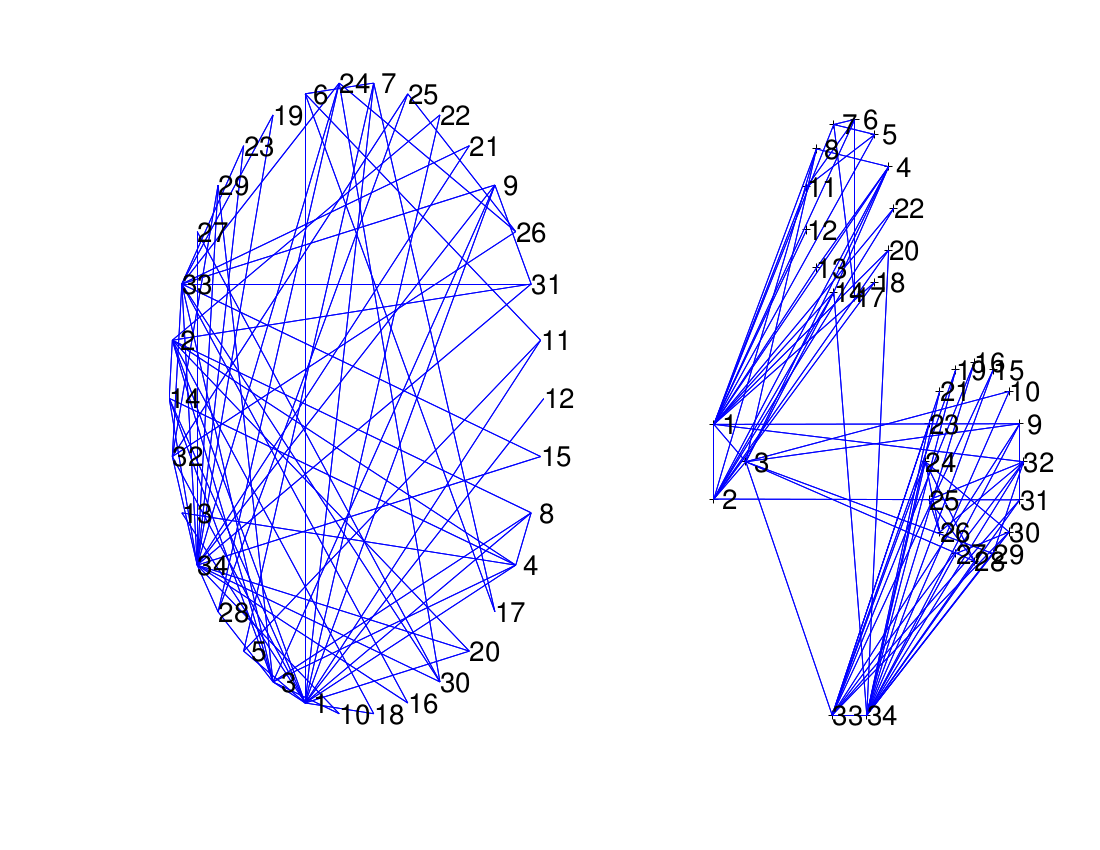
\epsfig{file =
      /RECHERCHE/RESEAUX/EXPOSES/FIGURES/Karate-Graph.eps, clip=, 
      width=8cm, height=10cm, angle=270, bbllx=75, bblly=475,
      bburx=530, bbury=770}
  \end{tabular}
\end{tabular}

%%%%%%%%%%%%%%%%%%%%%%%%%%%%%%%%%%%%%%%%%%%%%%%%%%%%%%%%%%%%%%%%%%%%%%%%
\newpage
\subsection{Existing results on random graphs}

\paragraph{Erd�s-Renyi model.} 
A huge amount of results about the behaviour of ER graphs regarding
\begin{itemize}
\vspace{-0.5cm}
\item the degree distribution (Poisson);
\vspace{-0.5cm}
\item the existence and the size of a giant component;
\vspace{-0.5cm}
\item the number of occurrences of motifs (Poisson and compound
  Poisson approximations);
\vspace{-0.5cm}
\item {\it etc.}
\end{itemize}
\vspace{-0.5cm}
\centerline{\paragraph{But ER fits very poorly most observed networks.}}

\bigskip
\paragraph{Generating functions.} 
Generating functions can be used to derive exact results such as the
distribution of the cluster size. 

As for sequences, such strategies are based on recursive properties and
require that the graph is 'tree like'.

\centerline{\paragraph{But biological networks are not tree-like.}}

%%%%%%%%%%%%%%%%%%%%%%%%%%%%%%%%%%%%%%%%%%%%%%%%%%%%%%%%%%%%%%%%%%%%%%%%
\newpage
\section{Some results for more general models}
%%%%%%%%%%%%%%%%%%%%%%%%%%%%%%%%%%%%%%%%%%%%%%%%%%%%%%%%%%%%%%%%%%%%%%%%

\noindent({\sl with E. Birmel�, J.J. Daudin, C. Matias,
  M. Mariadassou, F. Picard, E. Roquain, S. Schbath)}

\paragraph{Motif definition.}
A network motif of size $k$ ({\it ie} involving $k$ vertices)
is characterised by an adjacency matrix $\mbf$:
$$
\begin{tabular}{ll}
  \begin{tabular}{l}
    $m_{uv} = 1$ \\
    if an edge is required \\
    between nodes $u$ and $v$;  \\ 
    \\
    $m_{uv} = 0$  otherwise. \\ \\ \\ \\ \\ 
  \end{tabular}
  &
  $\begin{array}{ccccc}
    \mbox{Motif} & k & \mbf & \mbox{aut}(\mbf) & \rho(\mbf) \\
    \hline
    {\vee} & 3 & \left( {\small \begin{array}{ccc} 0&1&1\\&0&0\\&&0
        \end{array} } \right) & 2 & 3\\
    {\triangle} & 3 & \left(\small { \begin{array}{ccc} 0&1&1\\&0&1\\&&0
  \end{array} } \right) & 6 & 1\\
    {\square} & 4 & \left(\small { \begin{array}{cccc}
          0&1&0&1\\&0&1&0\\&&0&1\\&&&0 \end{array} } \right) & 8 & 3\\ 
  \end{array}$
\end{tabular}
$$
$\mbox{aut}(\mbf) = $ number of automorphism of $\mbf$. \\
$\Rcal(\mbf) = $ set of non-redundant permutations of $\mbf$;
$\rho(\mbf) = |\Rcal(\mbf)| = k! / \mbox{aut}(\mbf)$.

%%%%%%%%%%%%%%%%%%%%%%%%%%%%%%%%%%%%%%%%%%%%%%%%%%%%%%%%%%%%%%%%%%%%%%%%
\newpage
\paragraph{Occurrence of a motif.}
For any position $\alpha = (i_1, .. i_k)$  ($1 \leq i_1 < i_2 < ... < i_k
\leq n$), we define $Y_{\alpha}(\mbf)$:
$$
Y_{\alpha}(\mbf) 
= \Ibb\{\mbf \mbox{ occurs at } \alpha = (i_1, ..i_k)\} 
= \prod_{1 \leq u < v \leq k} X_{i_u i_v}^{m_{uv}}.
$$

\paragraph{Number of occurrences.} The count we are studying is
$$
N_{\wbf} = \sum_{\alpha} \sum_{\mbf' \in \Rcal(\mbf)} Y_{\alpha}(\mbf').
$$
The squared count is $ \displaystyle{N_{\wbf}^2 = \sum_{\alpha,
    \beta} \sum_{\mbf', \mbf'' \in \Rcal(\mbf)} Y_{\alpha}(\mbf')
  Y_{\alpha}(\mbf'')}.  $

\paragraph{Stationary hypothesis.}
We assume that the expectation of $Y_{\alpha}(\mbf)$ is the same all
over the graph:
$$
\Esp Y_{\alpha}(\mbf) = \mu(\mbf).
$$

% \paragraph{Occurrence probability.} The probability for $\mbf$ (or one
% of its permutated version) to occur at any position $\alpha$ is
% $$
% \sum_{\mbf' \in \Rcal(\mbf)} \Esp Y_{\alpha}(\mbf') =
% \sum_{\mbf' \in \Rcal(\mbf)} \mu(\mbf') =
% \rho(\mbf) \mu(\mbf).
% $$


%%%%%%%%%%%%%%%%%%%%%%%%%%%%%%%%%%%%%%%%%%%%%%%%%%%%%%%%%%%%%%%%%%%%%%%%
\newpage
\subsection{Mean and variance of the count}

\hspace{-2cm}
\begin{tabular}{cc}
  \begin{tabular}{p{10cm}}
    $
    \Esp N(\mbf) = \binom{n}{k} \rho(\mbf) \mu(\mbf).
    $
    \\ \\
    $\Esp N^2(\mbf) =$ \\
    $\displaystyle{\sum_{s=0}^{k} \left[ \binom{n}{k-s, s, k-s}
      \right. }$ \\
    $\displaystyle{\qquad \left. \sum_{\mbf', \mbf'' \in  \Rcal(\mbf)}
    \mu(\mbf'\underset{s}{\Omega} \mbf'') \right]}   
    $ \\  \\ \\
    \paragraph{On the right:} \\
    Star with 4 spikes ($k=5$): \\
    \begin{tabular}{cc}
      \begin{tabular}{c} $\mbf = $ \end{tabular} & 
      \begin{tabular}{c} \hspace{-2cm}     
\epsfig{file =
          /RECHERCHE/RESEAUX/EXPOSES/FIGURES/Motif-Star4.eps, clip=,
          width=2cm, height=2cm} 
      \end{tabular}   
    \end{tabular} \\
    All possible overlaps with $s=3$ nodes:
    $\mbf'\underset{3}{\Omega}\mbf''$. 
  \end{tabular}
  &
  \begin{tabular}{c}
    \epsfig{file=
      /RECHERCHE/RESEAUX/Motifs/FIGURES/MotifStar4-Recouv3.eps,
      clip, width=12cm, height=15cm}
  \end{tabular}
\end{tabular}



%%%%%%%%%%%%%%%%%%%%%%%%%%%%%%%%%%%%%%%%%%%%%%%%%%%%%%%%%%%%%%%%%%%%%%%%
\newpage
\subsection{Approximate distribution}

Based on simulations and analogy with motif statistics in sequences,
we propose to use the \paragraph{compound Poisson distribution}
(Polya-Aepply) to approximate the distribution of $N_{\mbf}$.

\hspace{-2cm}
\begin{tabular}{cc}
  \begin{tabular}{p{12cm}}
    The parameters of this distribution are derived from $\Esp
    N_{\mbf}$ and $\Var N_{\mbf}$: \\  
    \\
    \paragraph{Example:}  
    Distribution of the number of loops with 4 nodes ($\square$) 
    in a graph of size $n=200$, 
    under ERMG model with $Q=2$ groups and parameters 
    $$
    \alphabf = [\begin{array}{cc} 0.9 &  0.1 \end{array} ],
    \Pibf = \left[ \begin{array}{cc}
        0.004 & 0.037 \\ 
        0.037 & 0.004
      \end{array} \right].
    $$
    \\
  \end{tabular}
  &
  \begin{tabular}{l}
  $a = (\Var N_{\mbf}-\Esp N_{\mbf}) / (\Var N_{\mbf}+\Esp N_{\mbf}),$
  \\
  $\lambda = (1-a) \Esp N_{\mbf}$ \\
  \\
  \hspace{-1.3cm}
    \epsfig{file=/RECHERCHE/RESEAUX/Motifs/FIGJJD-150506/fig11_200.eps, 
      bbllx=332, bblly=211, bburx=515, bbury=304, width=12cm,
      height=7cm, clip=} \\
    \textred{\bf ---} Gaussian, \textgreen{\bf ---} Compound Poisson, 
%    \epsfig{file=
%        /RECHERCHE/RESEAUX/Motifs/FIGURES/DistStar4.eps, clip=,
%        width=14cm, height=12cm} 
   \end{tabular}
\end{tabular}
% The motif $\mbf = \square$ may occur at $\coefbin{200}{4} = 65\;10^6$
% positions. \\
We get 
$$
\Esp N_{\mbf} = 7.3, \qquad \Var N_{\mbf} = 21.7
$$
Suppose we observe 20 occurrences: $ \Pr\{N_{\mbf} \geq 20) \simeq 1.7
\%$. 

%%%%%%%%%%%%%%%%%%%%%%%%%%%%%%%%%%%%%%%%%%%%%%%%%%%%%%%%%%%%%%%%%%%%%%%%
\newpage
\section{Conclusions}

\paragraph{Sequences.} 
\begin{itemize}
\item \vspace{-0.5cm} Need for efficient computational techniques
  to study complex and/or fuzzy motifs. \\
  $\rightarrow$ (statistical, ) algorithmic, combinatoric, numerical
  issues
\item \vspace{-0.5cm} Need for models accounting not only for the
  primary information (nucleotide composition), but also for the
  secondary and tertiary (spatial configuration of the molecule)
  structures.
\end{itemize}

\paragraph{Networks.}
\begin{itemize}
\item \vspace{-0.5cm} Need for models $\left\{
    \begin{tabular}{p{17cm}}
      Fitting observed networks reasonably well, \\
      With parameters reasonably easy to estimate, \\
      Involving reasonably complicated combinatorics for the motifs.
      \end{tabular} \right. $
\item \vspace{-0.5cm} Need for probability and statistics to provide exact or
  approximate distributions. 
\item \vspace{-0.5cm} Need for computer science and algorithmics
  to calculate all this.
\end{itemize}

%%%%%%%%%%%%%%%%%%%%%%%%%%%%%%%%%%%%%%%%%%%%%%%%%%%%%%%%%%%%%%%%%%%%%%%%
%%%%%%%%%%%%%%%%%%%%%%%%%%%%%%%%%%%%%%%%%%%%%%%%%%%%%%%%%%%%%%%%%%%%%%%%
%%%%%%%%%%%%%%%%%%%%%%%%%%%%%%%%%%%%%%%%%%%%%%%%%%%%%%%%%%%%%%%%%%%%%%%%
%%%%%%%%%%%%%%%%%%%%%%%%%%%%%%%%%%%%%%%%%%%%%%%%%%%%%%%%%%%%%%%%%%%%%%%%
\end{document}
%%%%%%%%%%%%%%%%%%%%%%%%%%%%%%%%%%%%%%%%%%%%%%%%%%%%%%%%%%%%%%%%%%%%%%%%
%%%%%%%%%%%%%%%%%%%%%%%%%%%%%%%%%%%%%%%%%%%%%%%%%%%%%%%%%%%%%%%%%%%%%%%%
%%%%%%%%%%%%%%%%%%%%%%%%%%%%%%%%%%%%%%%%%%%%%%%%%%%%%%%%%%%%%%%%%%%%%%%%
%%%%%%%%%%%%%%%%%%%%%%%%%%%%%%%%%%%%%%%%%%%%%%%%%%%%%%%%%%%%%%%%%%%%%%%%

